
\begin{table}
\caption{Logical Operators per query for SqlPile and TPC-[H, DS] benchmarks. The SQLPile queries are far less complex.}
\label{tab:op-usage}
\begin{tabular}{lccc}
\toprule
\textbf{Operator} & \textbf{SqlPile} & \textbf{SQLStorm} & \textbf{TPC-[H, DS]} \\
\midrule
Projection & 1.264 & 3.613 & 4.000 \\
Scan & 0.750 & 4.171 & 4.050 \\
Filtered Scan & 0.386 & 1.200 & 3.142 \\
Join & 0.253 & 4.473 & 6.042 \\
Filter & 0.240 & 0.883 & 1.233 \\
Order By & 0.124 & 1.015 & 0.892 \\
Ungrouped Aggregate & 0.105 & 0.293 & 0.717 \\
Grouped Aggregate & 0.071 & 1.540 & 1.542 \\
Window Function & 0.004 & 0.581 & 0.175 \\
\bottomrule
\end{tabular}
\end{table}


We analyzed the operator usage of SqlPile queries and compared them to the TPC-H and TPC-DS benchmarks. As depicted in 
\cref{tab:op-usage}, SqlPile queries use far fewer logical operators than the TPC benchmarks.
This comes from the fact that a lot of the queries in SqlPile are simple \texttt{SELECT} statements from a transactional workload,
while the TPC benchmarks resemble an analytical workload with complex joins and aggregations.

\begin{table}
\caption{Most common logical column types of the tables in SqlPile. Fir SqlPile, the most columns are of type \texttt{Text} while for TPC-[H, DS] benchmarks, the most common type is \texttt{Integer}.}
\label{tab:column-types}
\begin{tabular}{lccc}
\toprule
\textbf{Logical Type} & \textbf{SqlPile} & \textbf{SQLStorm} & \textbf{TPC-[H, DS]} \\
\midrule
Text & 42.50\% & 36.56\% & 35.80\% \\
Int & 40.73\% & 45.96\% & 42.80\% \\
DateTime & 8.64\% & 3.96\% & 3.09\% \\
Float & 3.45\% & 13.07\% & 18.31\% \\
OTHER & 2.48\% & NaN & NaN \\
\bottomrule
\end{tabular}
\end{table}


We analyzed the distribution of logical column types used in SqlPile, which are shown in \cref{tab:column-types}, which is 
similar to findings in Redset~\cite{van_renen_why_2024} and the Public BI~\cite{vogelsgesang_get_2018} benchmark.

\begin{figure}
  \centering
  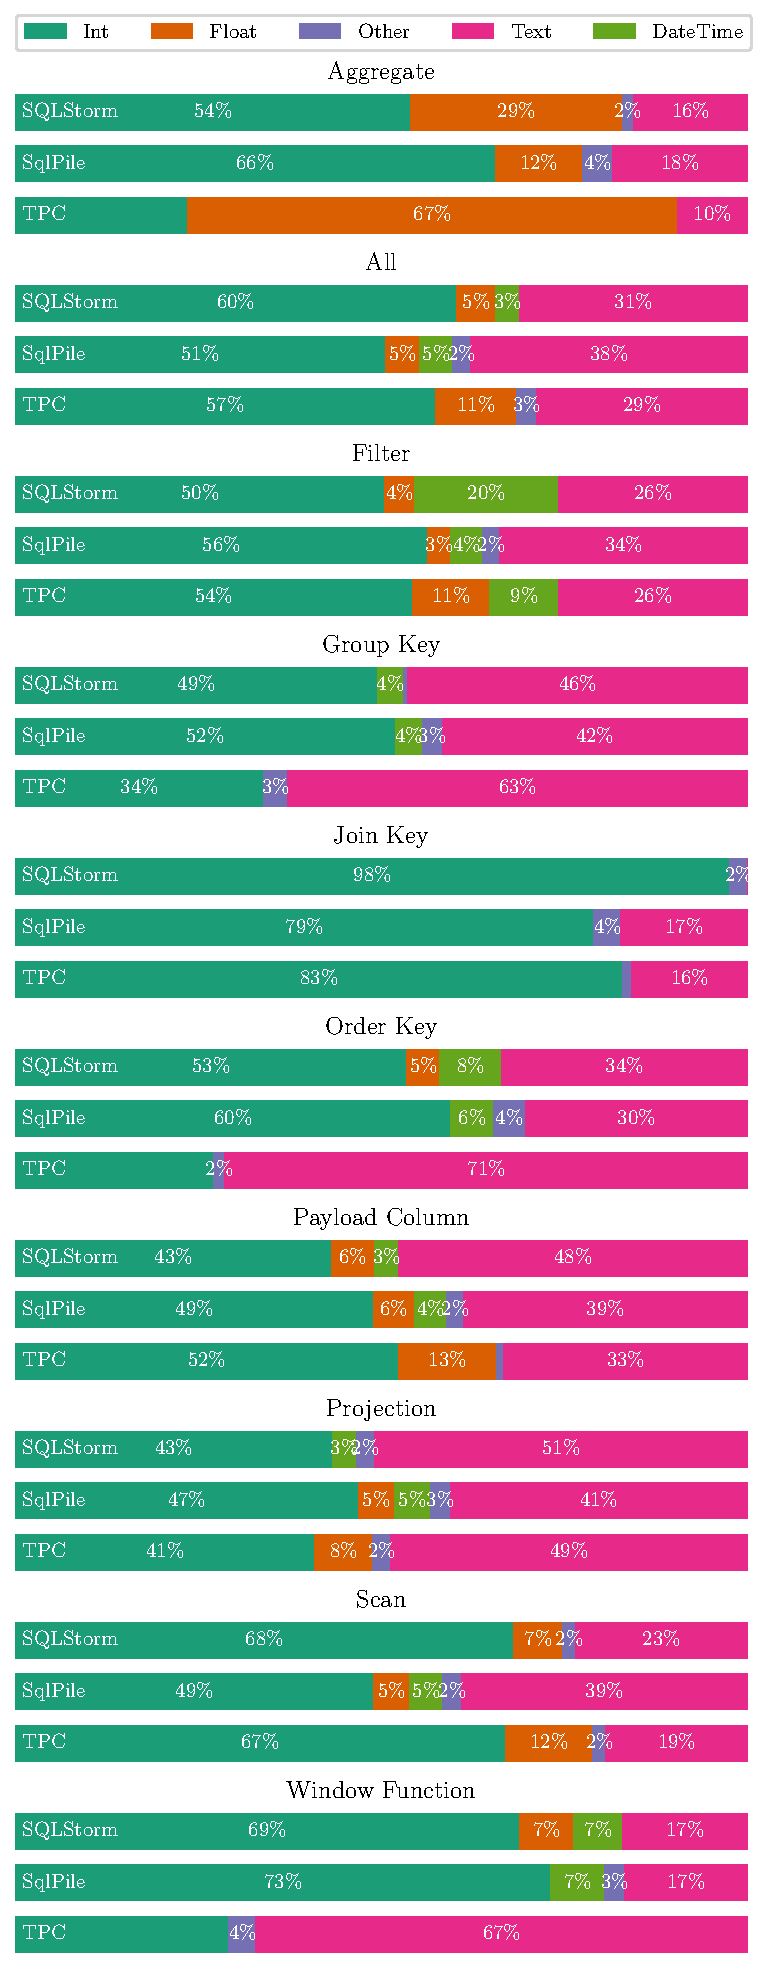
\includegraphics[width=\linewidth]{assets/column_usage/physical_type/column_cnt.pdf}
  \caption{Distribution of physical column types in SqlPile.}
  \Description{Distribution of physical column types in SqlPile.}
    \label{fig:column-physical-type-usage}
\end{figure}
